\documentclass{standalone}
\usepackage{tikz}
\usetikzlibrary{shapes.geometric}
\usetikzlibrary{patterns, positioning}
\usetikzlibrary{shapes.misc}
\usepackage[outline]{contour}
\contourlength{1.5pt} 


\begin{document}
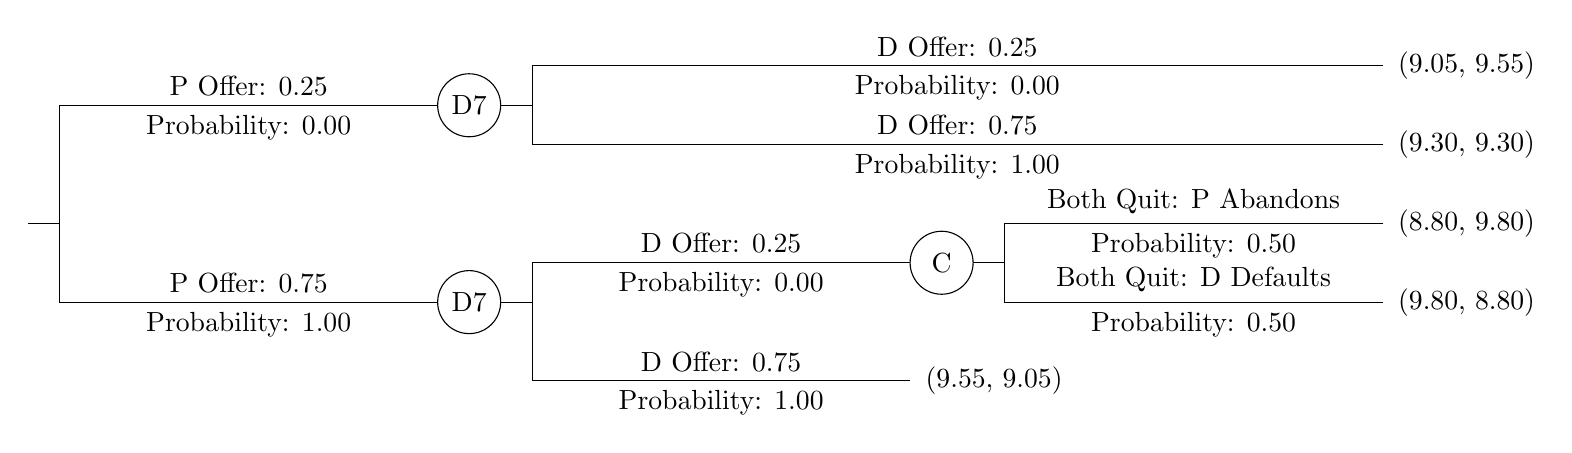
\begin{tikzpicture}

    \draw[color=black] (-12, -0.75) circle (0.4cm) node[draw=none] (N0) {D7};
\draw (-17.6, -2.25) -- (-17.200000000000003, -2.25) -- (-17.200000000000003, -0.75) -- (-12.4, -0.75) node [midway, above, sloped] (E0) {P Offer: 0.25} node [midway, below, sloped] (E1) {Probability: 0.00} ;


    \draw[color=black] (0, -0.25) node[draw=none] (N2) {};
\node[draw=none, right=-0.45cm of N2] {(9.05, 9.55)};
\draw (-11.6, -0.75) -- (-11.2, -0.75) -- (-11.2, -0.25) -- (-0.4, -0.25) node [midway, above, sloped] (E2) {D Offer: 0.25} node [midway, below, sloped] (E3) {Probability: 0.00} ;


    \draw[color=black] (0, -1.25) node[draw=none] (N4) {};
\node[draw=none, right=-0.45cm of N4] {(9.30, 9.30)};
\draw (-11.6, -0.75) -- (-11.2, -0.75) -- (-11.2, -1.25) -- (-0.4, -1.25) node [midway, above, sloped] (E4) {D Offer: 0.75} node [midway, below, sloped] (E5) {Probability: 1.00} ;


    \draw[color=black] (-12, -3.25) circle (0.4cm) node[draw=none] (N6) {D7};
\draw (-17.6, -2.25) -- (-17.200000000000003, -2.25) -- (-17.200000000000003, -3.25) -- (-12.4, -3.25) node [midway, above, sloped] (E6) {P Offer: 0.75} node [midway, below, sloped] (E7) {Probability: 1.00} ;


    \draw[color=black] (-6, -2.75) circle (0.4cm) node[draw=none] (N8) {C};
\draw (-11.6, -3.25) -- (-11.2, -3.25) -- (-11.2, -2.75) -- (-6.4, -2.75) node [midway, above, sloped] (E8) {D Offer: 0.25} node [midway, below, sloped] (E9) {Probability: 0.00} ;


    \draw[color=black] (0, -2.25) node[draw=none] (N10) {};
\node[draw=none, right=-0.45cm of N10] {(8.80, 9.80)};
\draw (-5.6, -2.75) -- (-5.199999999999999, -2.75) -- (-5.199999999999999, -2.25) -- (-0.4, -2.25) node [midway, above, sloped] (E10) {Both Quit: P Abandons} node [midway, below, sloped] (E11) {Probability: 0.50} ;


    \draw[color=black] (0, -3.25) node[draw=none] (N12) {};
\node[draw=none, right=-0.45cm of N12] {(9.80, 8.80)};
\draw (-5.6, -2.75) -- (-5.199999999999999, -2.75) -- (-5.199999999999999, -3.25) -- (-0.4, -3.25) node [midway, above, sloped] (E12) {Both Quit: D Defaults} node [midway, below, sloped] (E13) {Probability: 0.50} ;


    \draw[color=black] (-6, -4.25) node[draw=none] (N14) {};
\node[draw=none, right=-0.45cm of N14] {(9.55, 9.05)};
\draw (-11.6, -3.25) -- (-11.2, -3.25) -- (-11.2, -4.25) -- (-6.4, -4.25) node [midway, above, sloped] (E14) {D Offer: 0.75} node [midway, below, sloped] (E15) {Probability: 1.00} ;


\end{tikzpicture}
\end{document}